
\chapter{Experimental Results} % Main chapter title

\label{Chapter5} % For referencing the chapter elsewhere, use \ref{Chapter1} 


\lhead{Chapter 5. \emph{Experimental Results}} % This is for the header on each page - perhaps a shortened title


\section{Experimental Setup}

	Experiments evaluated the area and performance overhead of fingerprinting system compared with alternatives that utilize (a) software voting or (b) strict lockstep execution.
	Circuit size and complexity were evaluated by considering the resource utilization of each of the three systems when synthesized using Nios cores targeting an Altera Arria V FPGA development board.
	
	We first synthesized an implementation of the three-core architecture illustrated in Figure~\ref{f:arch}.
	One Nios core stands in for the fault tolerant core (FTC);
		we do not take steps to harden it.
	Note that safety-critical versions of the Nios and Microblaze cores are available for license~\cite{alteraniossc}\cite{xilinx_lockstep};
		these cores could act as a monitor with improved fault tolerance over a standard core.
	The architecture of the software voting system is the same as that used for fingerprinting;
		all logic supporting fingerprinting and fingerprint comparison is disabled, and redundancy checking is performed once at the end of the task, in software.
	We also synthesized a single core system to estimate the performance of a platform with a single lockstep pair as a baseline for comparison against fingerprinting and software voting.
	An actual lockstep system would likely have lower performance, as comparison logic of some sort is likely on the critical path.
	The development of a standalone lockstep system is beyond the scope of this work.
	
	First, we investigated the performance overhead of fingerprinting using benchmarks from the automotive suite from MiBench~\cite{guthaus2001mibench}.
	We modified each of basicmath, bitcount, qsort, and susan corners for execution on our fingerprinting system;
		the different benchmarks represent tasks of different lengths, input and output sizes, and store densities.
	Each benchmark repeatedly performed a calculation and we shortened the benchmarks by adjusting the number of times the main loop iterated.
	The size of the input data for qsort and susan were shortened to fit in the scratch-pad memory.
	Developing a comprehensive scratch-pad (or locked cache) allocation strategy and implementation that balances data size and algorithm complexity against fault containment is a potential subject for future investigation.
	
	The lockstep system may execute each benchmark directly;
		no manipulation to accommodate task duplication is needed.
	For each of fingerprinting and software voting, the task must first be duplicated on the pair of unreliable cores by the fault-tolerant monitor core.
	This is handled with a simple task graph transformation.
	In the case of fingerprinting, the task is replicated;
		no voting task is needed because fingerprinting and comparison hardware manage voting and report directly to the FTC.
	In the case of software voting, an additional voting task, dependent on each replicated task, is inserted, and performed by the FTC.

	Next, we performed a proof-of-concept evaluation of error detection latency under fingerprinting for each of the same four benchmarks.
	In order to demonstrate the error detection capabilities of fingerprinting we inject an error at the software level by corrupting, in software, a single value in the inputs to one of the two redundant tasks.
	When measuring error detection latency, we pessimistically assume that the effect of the faulty input propagates immediately into the execution stream (in reality it takes some time before the faulty input value is read, processed, and passed through the fingerprinting system).

	We do not attempt to perform an exhaustive fault injection campaign or to characterize the performance of the CRC algorithm or CRC based fingerprinting as an error detection mechanism; prior work has already addressed these issues.
	A table of 32 bit CRC polynomials and their associated hamming distances (i.e. minimum number of bits for which an error can go undetected) over various ranges of message length is given by Koopman in ~\cite{koopman200232}.
	Error detection latencies and probabilities with CRC-based fingerprinting was studied by Liu et al. in \cite{Meyer:13} through a simulation-based fault injection campaign of 1 and 2 bit data corruptions to a PowerPC register file.
	
	
\section{Results}
\label{s:results}

\subsection{Resource Utilization}

	We compare the cost in logic cells, registers and memory (in bits) of the main components of the fingerprinting system allocated to each unreliable core in Figure \ref{f:pie}(a).
	The Nios II figure includes a 1kB instruction cache and memory protection unit.
	Within a single core (we define the core as the CPU and any peripherals for which the CPU has its own copy), the fingerprint unit utilizes 16\% in combinationals, 14\% in registers, and less than 1\% in memory. We do not count the uTLB and DMA directly as overhead because they are peripherals that can be leveraged by other functions unrelated to reliability (and fingerprinting can technically be accomplished without them).
	%\bmtodo{Here's the place to say something about the simplicity of the Nios II core.  Can we make a comparison against a LEON3 core, too?  We should also state that the size of the logic doesn't change as the core changes, as the fingerprinting system is  entirely external to the core it is monitoring.}

\begin{figure}[tb]
\centering
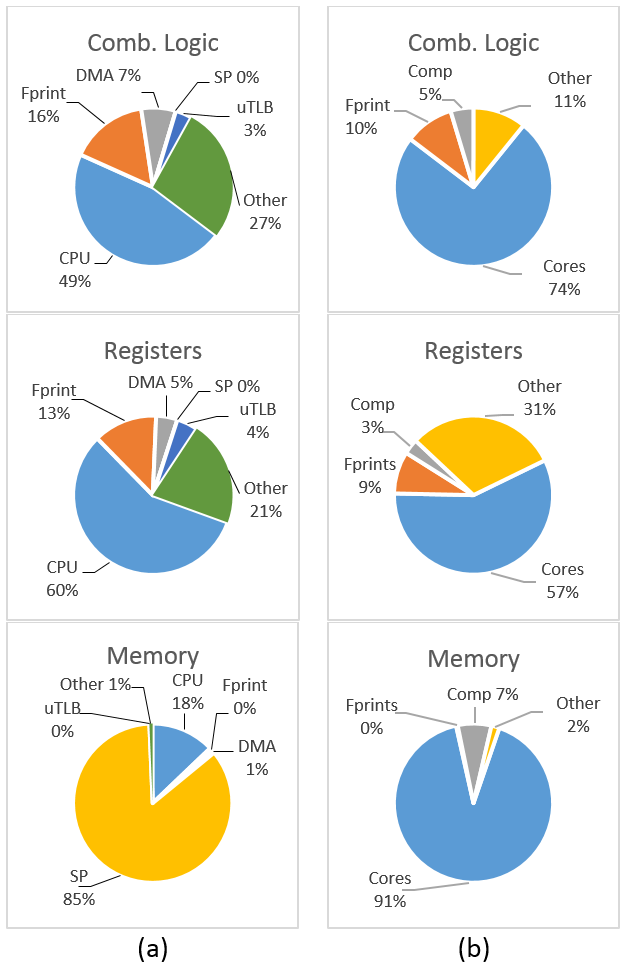
\includegraphics[scale=0.5]{figures/pie.png}
\caption[Fingerprinting FPGA resource allocation]{Fingerprinting FPGA overhead: (a) The local core and peripherals (b) The global system overhead}
\label{f:pie}
\end{figure}

	Figure \ref{f:pie}(b) shows the total cost of fingerprinting within a three core system where one core is assumed to be a reliable monitor and the two other cores are capable of fingerprinting.
	Therefore there are two fingerprinting units and a comparator added to the system.
	We note that the cost of the monitor core is probably too low because we have not implemented hardening or redundancy;
		this makes the relative cost of fingerprinting in this case pessimistic.
	The comparator represents only 6\% of combinationals, 4\% of registers and 7\% of onchip memory (excluding main memory).
	Note that the comparator is constant cost so long as the number of cores is less than 16, making this an upper limit cost;
		fingerprinting becomes more affordable the larger the number of cores that are supported.


\subsection{Single Task Replication and Detection Latency}

\begin{figure}[tb]
\centering
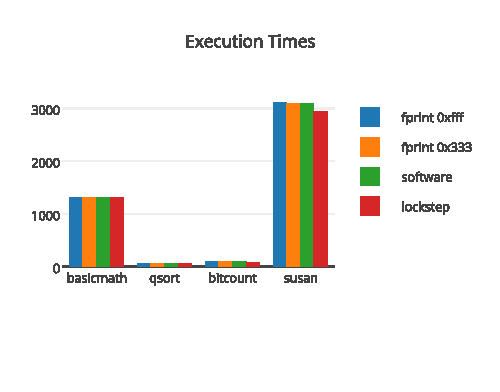
\includegraphics[scale=1.5]{Figures/execution_times}
\caption[Execution Time Results.]{\emph{Execution Time Results:} Four testbenches are executed on the three platforms. Fingerprinting is repeated with two different block sizes. There are no significant differences in execution time between any of the platforms.}
\label{f:extimes}
\end{figure}

	We compare the execution time of (a) lockstep DMR, (b) software voting, and (c) fingerprinting in Figure~\ref{f:extimes}.
	Fingerprinting is tested with two different block sizes.
	Execution time is measured from when the monitor first starts preparing the context of the other cores until it is notified that the task is completed, either by the comparator (under fingerprinting) or by the core themselves (under software voting).
	The performance of the fingerprinting and software checking platforms vary by less than 1\% for basicmath to 22\% for bitcount compared to the single core. The difference in execution time between fingerprinting and software checking is less than 1\% in all cases.
	The performance overhead associated with software checking and extra memory transactions (due to the fact that results must be copied from both cores) are not significant given the size of the data transfers compared to the lengths of the tasks.


\begin{figure}[tb]
\centering
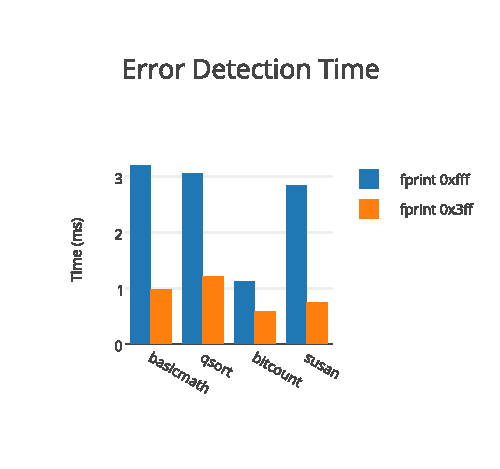
\includegraphics[scale=1.5]{Figures/error_detection_time}
\caption[Error detection latency]{The time it takes to detect an error with fingerprinting. Software voting cannot detect a fault until the task completes; lockstep DMR error detection latency varies based on implementation, but in some cases is no faster than fingerprinting.}
\label{f:dettimes}
\end{figure}

	In Figure~\ref{f:dettimes}, we report the error detection latency when one of the fingerprinted tasks is presented a faulty input.
	We observe that, as expected, the length of the fingerprinting block has an impact on detection latency.
	However, the placement of an error within a block and the density of store instructions will also have an effect.
	The bitcount testbench has such a different profile compared to the others because it uses bitwise operations as opposed to floating point which results in much more frequent pushing of data onto the stack. Furthermore, the erroneous input takes longer to affect the program execution.
		The detection latencies in Figure~\ref{f:dettimes} are significantly shorter than the execution times for a completed task; there is a potential to recover tens or even hundreds of extra milliseconds compared to software voting if a fault that occurs early in the execution of a task.
	
\subsection{Discussion}
	
	Consider again the Freescale Qorriva MPC577xK \cite{freescale2014qorivva} and Infineon Aurix 9x automotive ECUs \cite{infineon2014aurix} to place the resource utilization results in context. Firstly, a large amount of chip area on ECUs is devoted to interfacing with the external system. The Aurix chip, which is meant to be suited for several automotive applications that typically would have specialized ECUs, uses several serial bus controllers (e.g. I2C and Flex CAN), memory controllers, time management resources, interconnect logic, ADCs, and hardware security module. Secondly, the cores themselves are quite large and featured. The Qorriva Z7 cores have 16kB of instruction and data cache, 64 kB for data scratchpad, and FPUs. The lockstep functional safety core is also equipped with an FPU. Within this context, a fingerprint unit size of 30\% of the Nios core is quite reasonable. The Nios core we use has a 16kB scratchpad, 1kB instruction cache, no data cache or integer multiplication or division units and no MMU (future mixed criticality systems should expect to have full virtualization services to support hypervisors and more full-featured OS kernels such as Linux or Android). We argue that the comparison of fingerprint and CPU resource utilization on FPGA serves strictly as a rough measure demonstrating that the fingerprint unit is reasonably sized compared to the CPU and other peripherals that one might expect to find associated with each core. Furthermore, the size of comparator is reasonable taken against the size of the system when we consider that it supports up to 16 cores and that a realistic multicore ECU would be significantly larger than our prototype. Our platform excludes many peripherals and controllers such as IO interfaces, serial communication and memory controllers, ADC, PLL etc. 
	
	There are advantages to fingerprinting compared to core hardening techniques. While core hardening techniques exist that boast 10-15\% area overhead on custom CPU designs, they represent a a constant energy overhead whether the program running requires the higher reliability or not (i.e. they cannot be disabled). Furthermore, many core hardening techniques do not provide high enough coverage to support the most safety critical applications. Adoption of these techniques by manufacturers also poses a much greater risk since they require modifications to the CPU at the microarchitectural level. Fingerprinting is a non-invasive technique that can be integrated into a system without modifying the ISA or the CPU. Code can be written to be successfully fingerprinted without modifying the compiler toolchain or changing the code style from MISRA standards. We believe that fingerprinting is an ideal technique to be integrated into the automated design space exploration and code generation model-based design methodology because it provides several runtime tunable parameters and can be completely disabled.
	
	The main advantage of fingerprinting with respect to software checking and voting is the potential to greatly reduce detection latencies. Task level software checking suffers from large detection latency and increased memory transactions (although in the testbenches we examined these extra memory transactions were negligible). Single threaded software checking implemented by the compiler causes performance of the task to suffer and requires toolchain support (not tested in this paper but shown elsewhere). Multicore fault tolerant schedules require contingency plans in the case of failure. Fingerprinting reduces detection latencies which should eliminate the need for task grouping (which is done to reduce the overhead of voting and checking tasks) and can simplify the search for alternative schedules in the presence of multiple faults. Fingerprinting also has little to no impact on the performance of the task. Fingerprinting may cause very minor interference if it must use global buses to send information to the comparator. However these effects should be mitigated in a system with a deterministic (e.g. TDM) bus policy.	 
	
	
